\documentclass[12pt,UTF8]{ctexbook}
\usepackage{ctex}
\usepackage{caption}
\usepackage{graphicx}
\usepackage{float}
\usepackage{wrapfig}
\usepackage{array}
\usepackage[table, dvipsnames, svgnames, x11names]{xcolor}
\usepackage{colortbl}% 
\usepackage{tabularx}
\usepackage{amsmath, tikz}
\usepackage{amssymb}
\usepackage{xfrac}
\usepackage{eucal}
\usepackage{titlesec}
\usepackage{amsthm}
\usepackage{tikz-cd}
\usepackage{enumitem}
\usepackage{verbatim}
\usepackage{fontspec,xunicode,xltxtra}
\usepackage{xeCJK} 

\definecolor{gl}{RGB}{246, 252, 240}
\definecolor{gd}{RGB}{236, 244, 230}
\definecolor{bg}{RGB}{242, 244, 228}


\setCJKmainfont[BoldFont=STZhongsong]{STSong}
\setCJKmonofont{simkai.ttf} % for \texttt
\setCJKsansfont{simfang.ttf} % for \textsf
\setlength\parskip{8pt}
\setlength{\fboxsep}{12pt}
\renewcommand\thesection{\arabic{chapter}.\arabic{section}}

\usetikzlibrary{calc,topaths}

\newcommand\widearc[1]{%
\tikz[baseline=(wideArcAnchor.base)]{
    \node[inner sep=0] (wideArcAnchor) {$#1$}; 
    \coordinate (wideArcAnchorA) at ($(wideArcAnchor.north west) + (0.15em,0.1em)$);
    \coordinate (wideArcAnchorB) at ($(wideArcAnchor.north east) + (0.0em,0.1em)$);
%
    \draw[line width=0.1ex,line cap=round,out=45,in=135] (wideArcAnchorA) to (wideArcAnchorB);
}}

\newtheorem{df}{定义}[section] 
\newtheorem{pp}{命题}[section]
\newtheorem{tm}{定理}[section]
\newtheorem{ex}{例子}[section]
\newtheorem{sk}{思考}[section]
\newtheorem{po}{公理}
\newtheorem*{so}{解答}
\newtheorem*{proof2}{证明}
\newtheorem{xt}{习题}[section]
\newtheorem{cor}{推论}[pp]
% 列举环境的行间距
\setenumerate[1]{itemsep=0pt,partopsep=0pt,parsep=0pt,topsep=0pt}
\setitemize[1]{itemsep=0pt,partopsep=0pt,parsep=0pt,topsep=0pt}
\setdescription{itemsep=0pt,partopsep=0pt,parsep=0pt,topsep=0pt}
\setlength{\intextsep}{2pt}%
\setlength{\columnsep}{2pt}%
% 新函数
\renewcommand\parallel{\mathrel{/\mskip-4mu/}}
% 章节字体大小
\titleformat{\section}{\zihao{-2}\bfseries}{ \thesection }{16pt}{}
% 封面
\title{\zihao{0} \bfseries 第五册}
\author{\zihao{2} \texttt{大青花鱼}}
% \date{\bfseries\today}
% \date{}
% 正文
\begin{document}
\maketitle
\tableofcontents
\newpage

\chapter{圆}

学习反比例函数和二次函数时,我们发现,就算是简单代数式定义的函数,它的图像也是我们无法手动画出的曲线。
曲线是比直线更复杂的形状。为了给我们今后研究各种曲线打下基础,以下我们研究一种简单的曲线:圆。

\section{圆的基本性质}
我们已经学过圆的概念。公理体系中,我们这样定义圆:平面上到定点$O$距离为定长的点的集合,是一个圆。
给定线段$XY$,到$O$的距离和$AB$等长的点构成一个圆。$O$叫做\textbf{圆心},
$XY$叫做圆的\textbf{半径},长度一般记为$r$,不至于混淆的时候,半径的长也简称为半径。

圆心为$O$、半径为$r$的圆,一般记为圆$(O, r)$或$\odot(O, r)$。
圆心$O$和另一点$P$确定的圆,一般记为圆$(O, P)$或$\odot(O, P)$。如果不在意半径,不至于混淆的情况下,
也可以简记为圆$O$。

平面上的点到$O$的距离小于$r$,就说它在圆内;如果等于$r$,就说它在圆上;如果大于$r$,就说它在圆外。

关于圆,我们有以下公理:
\begin{itemize}
    \item 直线和圆有两个交点,当且仅当直线有部分在圆内。
    \item 给定点$A$、$B$和线段$EF$、$GH$,如果$|EF| + |GH| > |AB| > \left||EF| - |GH|\right|$,
    那么总存在两点$P$、$Q$,使得$|AP| = |EF|$、$|PB| = |GH|$,$|AQ| = |EF|$、$|QB| = |GH|$。
    $P$、$Q$分别在直线$AB$两侧。
\end{itemize}
第一个公理说明直线与圆相交的条件,第二个公理则说明圆与圆相交的条件。

考虑直线$l$和圆$\odot(O, r)$。过$O$作直线$m\perp l$,记垂足为$P$,$|OP| = d$。

\begin{figure}[h] %this figure will be at the right
    \vspace{8pt}
    \centering
    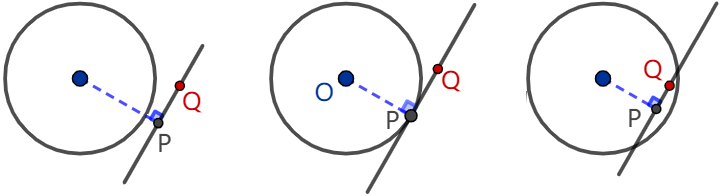
\includegraphics[width=0.72\textwidth]{圆与直线1.png}
\end{figure}

\begin{enumerate}
    \item 如果$d > r$,那么$P$在圆外。对$l$上任意其他点$Q$,根据勾股定理,$|OQ|^2 = |OP|^2 + |PQ|^2 > |OP|^2$,因此$|OQ| > |OP| > r$。这说明$l$上的点都在圆外。我们说直线$l$与圆$O$\textbf{相离}。反之,如果直线与圆相离,那么$P$在圆外,因此$d > r$。
    \item 如果$d = r$,那么$P$在圆上。对$l$上任意其他点$Q$,根据勾股定理,$|OQ|^2 = |OP|^2 + |PQ|^2 > |OP|^2$,因此$|OQ| > |OP| = r$。这说明$l$上其他点都在圆外。直线和圆恰有一个公共点。我们说直线$l$与圆$O$\textbf{相切},称$P$为\textbf{切点}。
    反之,如果直线与圆相切于点$Q$,那么$|OQ| = r$。反设$Q$不是$P$,那么根据勾股定理,$|OP|^2 = |OQ|^2 - |PQ|^2 < |OQ|^2$,这说明$P$在圆内。根据第一个公理,圆$O$和$l$有两个交点,矛盾!因此$Q$就是$P$,$d = r$。
    \item 如果$d < r$,那么$P$在圆内。根据第一个公理,直线和圆有两个交点$A$、$B$。我们说直线与圆\textbf{相交},或直线\textbf{割圆}于$A$、$B$。
    反之,如果直线和圆有两个交点,那么根据第一个公理,直线有部分在圆内。设$Q$在圆内,那么根据勾股定理,$|OP|^2 = |OQ|^2 - |PQ|^2 < |OQ|^2$,这说明$P$在圆内,即$d < r$。
\end{enumerate}
从以上的讨论可以看出,圆心到直线的垂足$P$,以及$OP$,是判断直线和圆关系的重要依据。

设直线割圆于两点$A$、$B$,根据第一个公理,线段$AB$(除端点)在圆内。
我们把线段$AB$称为圆的一条\textbf{弦}。
连接圆上一点$A$和圆心$O$,延长$AO$,根据第一个公理,它和圆有另一个交点$B$,称为点$A$的\textbf{对径点}。
$AB$称为圆的\textbf{直径}。直径是过圆心的弦。它的长度是半径的两倍。不至于混淆的时候,直径的长也简称为直径。

给定圆上两点$A$、$B$,考虑弦$AB$的垂直平分线$l$,圆心$O$显然在$l$上。也就是说,\textbf{恰有一条直径垂直平分每条弦}。

考虑两个圆:$\odot(O_1, r_1)$和$\odot(O_2, r_2)$,设两个圆心的距离是:$|O_1O_2| = s$,
那么,两个圆的关系可能有以下几种:

\begin{figure}[h] %this figure will be at the right
    \vspace{8pt}
    \centering
    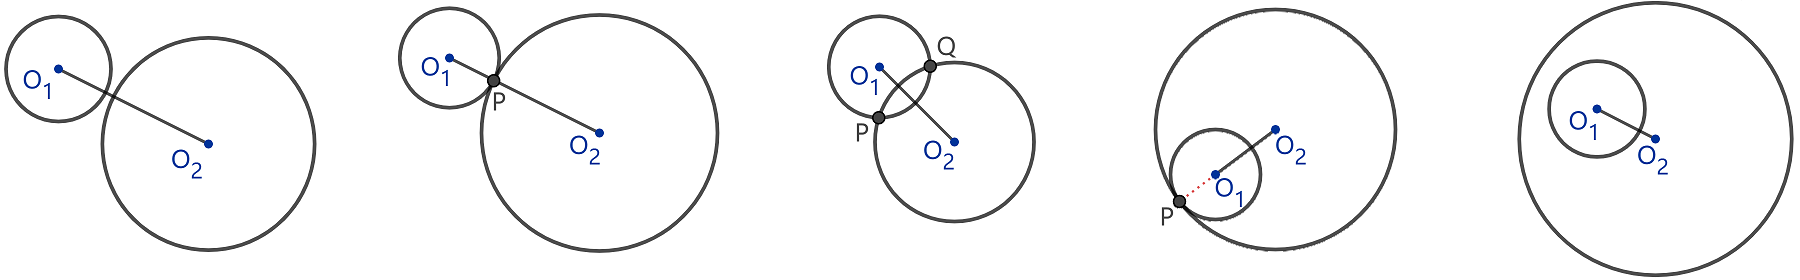
\includegraphics[width=0.9\textwidth]{圆与圆1.png}
\end{figure}

\begin{enumerate}
    \item $s > r_1 + r_2.$ 用反证法可以证明,两个圆没有公共点。我们说两圆\textbf{相离}。
    \item $s = r_1 + r_2.$ 考虑线段$O_1O_2$,上面有一点$P$使得$|O_1P| = r_1$,于是$|PO_2| = |O_1O_2| - |O_1P| = r_2$。
    这说明两个圆有一个公共点。如果点$Q$不在线段$O_1O_2$上,则$|O_1Q| + |QO_2| > |O_1O_2|$。
    于是$Q$不可能是公共点。也就是说,两个圆恰有一个共同点,在圆心连线上。我们说两圆\textbf{外切}。
    \item $|r_1 - r_2| < s < r_1 + r_2.$ 根据第二个公理,$\odot(O_1, r_1)$和$\odot(O_2, r_2)$恰有两个公共点,分别在圆心连线两侧。我们说两圆\textbf{相交}。
    \item $s = |r_1 - r_2|.$ $r_1 > r_2$时,$s = r_1 - r_2$。考虑直线$O_1O_2$,上面有一点$P$,使得$|O_1P| = r_1$,且和$O_2$在$O_1$同一边。于是$|O_2P| = |O_1P| - |O_1O_2| = r_2$。
    这说明两个圆有一个公共点。如果点$Q$不在线段$O_1O_2$上,则$|O_1O_2| + |QO_2| < |O_1Q|$。
    于是$Q$不可能是公共点。也就是说,两个圆恰有一个共同点,在圆心连线上。$r_1 > r_2$时,通过类似推理可以得到同样的结论。我们说两圆\textbf{内切}。
    \item $s < |r_1 - r_2|.$ 用反证法可以证明,两个圆没有公共点。如果$r_1 > r_2$,我们说$\odot(O_1, r_1)$\textbf{内含}$\odot(O_2, r_2)$,$\odot(O_2, r_2)$\textbf{容于}$\odot(O_1, r_1)$;反之亦然。
\end{enumerate}
要注意的是,如果仅知道两圆恰有一个公共点,我们无法判断到底是第二还是第四种情形;如果仅知道两圆没有公共点,我们无法判断到底是第一还是第五种情形。
第二和第四种情形可以统称为两圆\textbf{相切},第一和第五种情形可以统称为两圆\textbf{相离}。

\begin{xt}\label{xt:0-0-0}
    补充:\\
    \indent 1. 设直线割圆于两点$A$、$B$,证明线段$AB$(除端点)在圆内。\\
    \indent 2. 完成两圆关系的第一和第五种情形中的证明。\\
    \indent 3. 阐明两圆关系的第四种情形中,$r_1 > r_2$情况下的推理过程。
\end{xt}

\section{圆和旋转}
怎么画一个圆?我们用圆规画圆。如果已知圆心和圆上一点,我们将圆规尖定在要画的圆心处,
将笔头接触圆上的点,然后轻轻旋转,笔头就画出一个圆。如果已知圆心和半径线段,我们首先张开圆规,
圆规尖和笔头分别对齐半径两端,然后保持圆规形状不变,将圆规尖定在要画的圆心处,让笔头接触纸面,
轻轻旋转,笔头就画出一个圆。

可以看出,圆和旋转有天然的关系。旋转是由角定义的操作,把平面中的点映射到另一点。
给定角$AOB$,可以这样定义\textbf{旋转}:

\begin{df}\label{df:0-1-0}
    给定角$AOB$,平面中一点$P$关于$\angle AOB$旋转的结果,
    是唯一使得$\angle POQ = \angle AOB$且$|OP| = |OQ|$的点$Q$。
\end{df}
$O$称为旋转的\textbf{中心}。任何点$P$绕中心旋转,结果都在圆$(O,P)$上。

可以看到,给定一个圆$(O,P)$,从点$P$出发,旋转不同的角度,
就得到圆上其它的点。用圆规画圆时,从零角出发,随着角度不断增大,直到周角,我们沿逆时针经历了圆上所有的点
(注意:这里约定角度的范围是$0^\circ$到$369^\circ$)。
也就是说,我们认为零角到周角的角按角度和圆上的点之间有一一映射。
换句话说,数轴上$0$和$360$之间的数,和圆上的点之间有一一映射。
我们把它称作\textbf{圆映射},记为$\gamma_{(O,P)}$。

通过$\gamma_{(O,P)}$,我们可以把对圆的研究,改为对数轴上线段的研究。
这样就把曲线上的问题转为了直线上的问题。
比如,既然$[0, 360)$对应整个圆,那么$[0,180]$就对应半个圆,
$[0,60]$就对应六分之一个圆,等等。我们把闭区间对应的圆的部分称为\textbf{圆弧}。

同一圆上两个圆弧分别对应$[a_1, a_1+x]$和$[a_2, a_2+x]$,这两个圆弧有什么不同吗?
观察圆的图像可知,并没有不同。也就是说,圆弧的形状只和它对应数轴上区间的长度有关,和它所在的位置无关。
只要对应的区间一样长,那么圆弧就全等,可以相互覆盖。换句话说,圆弧只要等长,就是全等的。
于是,线段所满足的公理,对同一个圆上的圆弧也成立。

和线段一样,圆弧也有起点和终点。比如$[0,60]$对应的圆弧,起点就是$P$,
终点是$60$度角$POQ$的终边和圆的交点$Q$。如果圆弧对应的区间长度超过$180$,就说它是\textbf{优弧};
如果圆弧对应的区间长度小于$180$,就说它是\textbf{劣弧};如果等于$180$,就说它是\textbf{半圆}。
优弧比半圆长,劣弧比半圆短。

从直线和圆相交的角度来看,圆上两点表示这两点确定的直线将圆分为两个圆弧。这两个圆弧并起来就是圆,
所以要么一个是优弧、一个是劣弧,要么两者都是半圆(这时直线过圆心)。

同一个圆上,明确了起点$A$和终点$B$,就唯一确定了圆弧$\widearc{AB}$。如果只说了两点$A$、$B$,
那么$\widearc{AB}$一般指劣弧或起点为$A$终点为$B$的圆弧。如果要指优弧,一般会特别强调。

\begin{xt}\label{xt:0-1-0}
    证明:\\
    \indent 1. 同一个圆中,直径是最长的弦。\\
    \indent 2. 任意线段经过旋转得到等长的线段。任意三角形经过旋转得到同角全等的三角形。 
\end{xt}

\section{圆心角和圆周角}

根据圆映射的定义,每个圆弧都对应一个顶点在圆心,大小介于零角和周角之间的角,称为它的\textbf{圆心角}。
圆弧还可以对应另一类角。给定起点为$A$,终点为$B$的圆弧$\widearc{AB}$和圆上一点$P$,则角$APB$称为一个\textbf{圆周角}。
每个圆弧只对应一个圆心角,但可以对应很多个圆周角。

同一段圆弧的圆心角和圆周角之间,有什么关系呢?如右图,连接$PO$,延长交圆于对径点$Q$。
由于$\triangle AOP$是等腰三角形,$\angle OAP + \angle OPA = 0$,
同理,$\angle OBP + \angle OPB = 0$。于是
\begin{align}
    \angle AOB &= \angle AOQ + \angle QOB \notag \\ 
    &= \angle OAP + \angle APO + \angle PBO + \angle OPB \notag \\
    &= 2\angle APO + 2\angle OPB = 2\angle APB \notag
\end{align}
也就是说,圆心角是圆周角的两倍大小,圆周角是圆心角的一半大小。
由于每段圆弧只对应一个圆心角,无论$P$取圆上哪个点,只要不在弧上,圆周角$APB$都是圆心角的一半大小。

如果点$P$在弧上,$\angle APB$和$\angle AOB$是什么关系呢?如果点在弧上,它对应的就是构成圆的另一段弧,于是它
是另一段弧对应的圆心角的一般大小。另一段弧对应的圆心角是周角减去$\angle AOB$,所以
$$\angle APB = 180^\circ - \angle AOB.$$

\begin{tm}\textbf{圆周角定理}\label{tm:0-2-0}
    给定圆$O$上的弧$\widearc{AB}$及圆上的点$P$,如果$P \notin \widearc{AB}$,那么:
    $$\angle APB = \frac{1}{2} \angle AOB,$$
    如果$P \in \widearc{AB}$,那么:
    $$\angle APB = 180^\circ - \frac{1}{2} \angle AOB.$$
\end{tm}
对径点和圆心形成平角,因此,根据圆周角定理,对径点对应的圆周角是直角。或者说,半圆对应的圆周角是直角。

要注意的是,讨论圆心角时,我们约定角的范围是零角到周角。讨论圆周角和其他角时,为了方便,我们会切换到
负平角到正平角的范围。

同一个圆里,圆上的点$A$、$B$对应的圆心角$\angle AOB$和点$C$、$D$对应的圆心角$\angle COD$相等,那么
根据“边角边”,圆心$O$和它们构成的三角形满足:$\triangle AOB \simeq \triangle COD$。弦$AB$和$CD$也等长。
不仅如此,根据圆映射,圆弧$\widearc{AB}$和$\widearc{CD}$也等长。
事实上,$\widearc{CD}$就是$\widearc{AB}$关于某个角旋转的结果。
我们把这个结论称为“等角对等弦”、“等角对等弧”。

反之,如果两个圆弧$\widearc{AB}$和$\widearc{CD}$等长,那么它们对应的区间也一样长。
这说明它们对应的圆心角一样大。
圆心角既然相等,那么弦$AB$和$CD$也等长。
更进一步,设$P$是圆上不属于两弧的点,那么圆周角$\angle APB$和$\angle CPD$一样大。我们把这个结论称为“等弧对等弦”、“等弧对等角”。

反过来,如果圆$O$上两条弦$AB$和$CD$等长,那么根据“边边边”,$\triangle AOB \simeq \triangle COD$。
于是圆心角相等,所以劣弧$\widearc{AB}$和$\widearc{CD}$等长。我们把这个结论称为“等弦对等角”、“等弦对等弧”。

总的来说,在同一个圆里,两点对应的弦长相等当且仅当对应的(劣弧)弧长相等,当且仅当对应的圆心角相等,
当且仅当对应的圆周角相等。弦、弧、圆心角、圆周角,都是用来描述圆的部分和整体关系的方法。

给定圆上两点$A$、$B$,它们对应的垂直平分线$l$平分$\angle AOB$,即把$\angle AOB$分成两个相同大小的圆心角。
因此,设$l$和圆交于$P$、$Q$,则它们也分别平分所在的圆弧(称为弧的中点)。
我们把这一系列结论总称为垂径定理:
\begin{tm}\textbf{垂径定理 }\label{tm:0-2-1}
    给定圆上两点,则恰有圆的一条直径垂直平分两点对应的弦,同时平分对应的圆心角和两个圆弧。
\end{tm}
垂径定理也可以说成:过圆$O$的弦$AB$中点的直径与弦$AB$垂直,同时平分$\angle AOB$和弧$\widearc{AB}$。

\begin{xt}\label{xt:0-2-0}
    给定圆$O$,弦$AB$中点记为$M$,$|MO|$称为弦$AB$的\textbf{弦心距}。\\
    \indent 1. 证明:圆心角相等,当且仅当对应的弦心距相等。\\
    \indent 2. 设直线$MO$与圆$O$交于$P$、$Q$两点,证明:$|MP| \cdot |MQ| = |MA|\cdot |MB|.$
\end{xt}

\section{圆内接四边形}
我们对圆上一点、两点引出的形状都有了初步了解,现在来看圆上多个点对应的形状。首先来看三个点的情形。

设$A$、$B$、$C$是圆$(O,r)$上(相异的)三点,则线段$AB$、$BC$、$AC$的垂直平分线都过圆心$O$。
因此,$O$是$\triangle ABC$的外心(这里附带说明了圆上相异三点必然不共线),$|OA|=|OB|=|OC|=r$。
反之,设有(非退化的)$\triangle ABC$,以它的外心$O$为圆心,以$|OA|$为半径,就可以画出一个圆,
过顶点$A$、$B$、$C$。这说明,\textbf{不共线的三点恰好对应一个圆}。或者说,\textbf{不共线的三点确定一个圆}。
我们把这个圆称为三角形的\textbf{外接圆}(“外心”即“外接圆圆心”简称),把三角形称为圆的\textbf{内接三角形}。

在三个点的基础上再加一个点$D$,四个点$A$、$B$、$C$、$D$能否恰好对应一个圆呢?显然,
$\triangle ABC$和$\triangle BCD$的外接圆未必是同一个圆。所以,四个点不总是在同一个圆上。
换句话说,要让四个点共圆,这四个点必须满足一定的条件。

如右图上情形,设$A$、$B$、$C$、$D$圆$(O,r)$上(相异的)四点,考察它们对应的圆弧。我们发现,
$\widearc{ABC}$和$\widearc{CDA}$是整个圆的两部分,因此,它们对应的圆心角之和是周角。
根据圆周角定理,$\angle ABC + \angle CDA = 180^\circ$。同理,$\angle BCD + \angle DAB = 180^\circ$。

我们还可以发现,圆周角$\angle BAC$和$\angle BDC$都对应$\widearc{BC}$,因此根据“等弧对等角”,
$\angle BAC = \angle BDC$。同理可得:$\angle ACB = \angle ADB$,$\angle CAD = \angle CBD$,
$\angle DBA = \angle DCA$。从这些等角关系出发,
如果对角线$AC$和$BD$交于点$P$,那么$\triangle APB \backsim \triangle CPD$、$\triangle BPC \backsim \triangle DPA$。

如果$A$、$B$、$C$、$D$顺序改变,如右图下情形,那么$\widearc{ABC}$和$\widearc{CDA}$对应同一段圆弧$\widearc{AC}$。
这时$\angle ABC + \angle CDA = 0^\circ$,或者说$\angle ABC = \angle ADC$。
同理,$\angle BAD = \angle BCD$。
我们把这样的四边形$ABCD$称为\textbf{凹四边形},把前一种情况中的四边形$ABCD$称为\textbf{凸四边形}。
凸四边形包含我们学过的平行四边形、梯形和筝形,它的内角都是正的。凹四边形的内角总有负的。
无论是凸四边形还是凹四边形,内角和总是零角。

综合两种情况,\textbf{圆内接凸四边形对角之和是平角},\textbf{圆内接凹四边形对角相等}。

四边形$ABCD$有一对边相交,像一只蝴蝶。我们把这样的四边形叫做\textbf{蝶形}。可以看到,如果把相交的对边
$AB$、$CD$看作对角线,把对角线$AC$、$BD$看作对边,我们就得到一个凸四边形$ACBD$。
因此,观察相同的圆弧对应的圆周角可以发现,我们仍然有$\angle BAC = \angle BDC$、$\angle ACB = \angle ADB$,$\angle CAD = \angle CBD$,
$\angle DBA = \angle DCA$。如果对角线$AC$和$BD$交于点$P$,仍然有$\triangle APB \backsim \triangle CPD$、$\triangle BPC \backsim \triangle DPA$。

以上是圆内接四边形边和角的性质,反过来,满足什么性质的四边形是圆内接四边形呢?

\section{圆内接多边形}
从四边形的情况来看,顶点的位置顺序对形状很重要。如果顶点$A$、$B$、$C$、$D$按顺时针或逆时针顺序排列,
那么四边形$ABCD$是凸四边形,否则,四边形$ABCD$可能是凹四边形。

对一般的圆内接多边形,我们只研究最简单的一类:顶点按逆时针顺序排列的多边形。
具体来说,设圆$O$上有$n$个点:$A_1, A_2, \cdots , A_n$,从$A_1$出发构造圆映射$\gamma_{(O,A_1)}$,
把$[0, 360)$映射到圆周,那么$0$对应$A_1$。设$t_1, t_2, \cdots , t_n$分别对应$n$个点,
那么$0 = t_1 < t_2 < \cdots < t_n$。这样定义的圆内接多边形:$A_1A_2\cdots A_n$就是我们研究的对象。
这样定义的多边形,每个内角都在零角和平角之间。这样的多边形叫做\textbf{凸多边形}。

对于大于等于$3$的整数$n$,凸$n$边形$A_1A_2\cdots A_n$有$\frac{n(n-3)}{2}$条对角线。
具体来说,每个顶点和相邻两个顶点的连线是$n$边形的边,和其余$n-3$个顶点的连线是对角线。
因此每个点是$n-3$条对角线的端点。另一方面,每条对角线对应两个顶点,因此一共有$\frac{n(n-3)}{2}$条对角线。

凸多边形的内角和是否有规律呢?我们知道三角形的内角和是平角,凸四边形的内角和是两个平角
(或者说周角,如果把角度约定在负平角和正平角之间,则减去一个周角变成零角)。边数继续增多时,
我们定义凸$n$边形$A_1A_2\cdots A_n$的内角和为:

$$ \angle A_1A_2A_3 + \angle A_2A_3A_4 + \cdots + \angle A_{n-2}A_{n-1}A_{n} + \angle A_{n-1}A_{n}A_{1}+ \angle A_{n}A_{1}A_{2}$$

如果我们不把角度限定在负平角和正平角之间,可以猜测:凸$n$边形的内角和是$n-2$个平角。

如果凸多边形是圆内接多边形,我们可以这样证明:$n$个顶点把圆分为$n$段圆弧。每个顶点张成的内角,
对应了其中$n-2$段圆弧。如果考虑所有$n$个内角对应的圆弧,则每段圆弧计入$n-2$次(圆弧两端是内角顶点的时候不计入,
其它情况下都计入)。也就是说,$n$个内角和对应$n-2$个整圆。这些内角都是圆周角,
因此它们的和是$n-2$个整圆对应的圆周角,即$n-2$个平角。我们的猜想至少对圆内接多边形是正确的。

对一般凸多边形的情况,我们可以通过不断“裁剪”三角形来证明。我们还记得,凸四边形可以裁成两个三角形,
因此它的内角和是两个三角形的内角和。从另一个角度来看,我们通过裁掉一个三角形,把凸四边形变成了三角形。
对一般的凸$n$边形$A_1A_2\cdots A_n$来说,由于它的每个内角都介于零角和平角之间,我们可以考虑裁掉某个角,
把它变成$n-1$边形。比如,沿着线段$A_1A_3$剪一刀,
就把$A_1A_2\cdots A_n$分成了三角形$A_1A_2A_3$和$n-1$边形$A_1A_3\cdots A_n$。

\begin{tm}
    凸$n$边形的内角和是$n-2$个平角。
\end{tm}
\begin{proof2}
    用归纳法证明。命题$P(n)$:凸$n+2$边形的内角和是$n$个平角。我们要证明$P(n)$对所有正整数$n$成立。\\
    $n=1$时,由于三角形内角和是平角,$P(1)$成立。\\
    假设$P(n)$成立,下面证明$P(n+1)$成立。\\
    设有凸$n+3$边形$A_1A_2A_3\cdots A_n$,将它裁成三角形$A_1A_2A_3$和$n-1$边形$A_1A_3\cdots A_n$。
    前者的内角和是平角。根据$P(n)$,后者的内角和是$n$个平角,因此,$A_1A_2A_3\cdots A_n$的内角和是$n+1$个平角。
    于是$P(n+1)$成立。\\
    因此对所有正整数$n$,命题$P(n)$成立。
\end{proof2}

满足什么条件时,凸多边形是圆内接多边形呢?最直接的条件,自然是平面上有一个圆,
使多边形顶点都在圆上。或者说,能找到一点,到多边形各个顶点距离相等。

如果难以直接找到这样的点,可以查看多边形各边和各条对角线的垂直平分线。
如果多边形是圆内接多边形,它的边和对角线都是圆的弦,垂径定理说明其垂直平分线过圆心。
具体来说,可以考察两条边(或对角线)的垂直平分线的交点。这点如果到各个顶点距离相等,
那么多边形内接于以它为圆心的圆,否则多边形不是圆内接多边形。

有一种特殊的凸多边形必然是圆内接多边形:\textbf{正多边形}。
正多边形是各边等长,各内角相等的多边形。正三角形、正方形都是正多边形。
正多边形的内角角度是$\frac{180(n-2)}{n}^\circ$

\begin{xt}
    \mbox{}\\
    \indent 1. 平行四边形、矩形、正方形、梯形、筝形,哪些总是圆内接多边形?哪些可以是圆内接多边形?要满足什么条件?\\
    \indent 2. 设有整数$1 \leqslant i,j,k,l \leqslant n$,圆内接$n$边形$A_1A_2\cdots A_n$中,$\angle A_iA_kA_j$和$\angle A_iA_lA_j$有什么关系?
\end{xt}

\section{弧长和面积}


\chapter{圆和三角形}
\section{圆幂}
\section{切线和割线}
\section{垂心和外接圆}
\section{内切圆和旁切圆}
\section{九点圆}

\chapter{三角函数}
\section{锐角的三角函数}
\section{三角函数的图像和性质}
\section{三角函数和三角形}


\chapter{从或许到确定}
\section{事件和试验}
\section{计数和概率}
\section{组合和排列}

\chapter{三段论(上)}
\section{大前提、小前提和结论}
\section{直言三段论}

\end{document}